\documentclass{beamer}
\usepackage{pdfpages}
%Imports and customization
\usepackage{tikz}
\usepackage{graphicx}
\usepackage{tikz-feynman}
\usepackage{ulem}
\usepackage{colortbl}
\graphicspath{ 
    {./images/}
}

\beamertemplatenavigationsymbolsempty
\setbeamertemplate{sidebar right}{}
\setbeamertemplate{footline}{
    \hfill\usebeamertemplate***{navigation symbols}
    \hspace{1cm}\insertframenumber{}/\inserttotalframenumber
}
\setbeamertemplate{caption}{\raggedright\insertcaption\par}
\setbeamersize{text margin left=4mm,text margin right=4mm} 

\setbeamerfont{itemize/enumerate body}{size=\scriptsize}
\setbeamerfont{itemize/enumerate subbody}{size=\scriptsize}
\setbeamerfont{itemize/enumerate subsubbody}{size=\scriptsize}


%Custom Macros
\newcommand{\statwarn}{
    \tiny \color{red} Absolute numbers here mean NOTHING. Plots are based on small (100k events) samples, and are highly biased. All that matters is relative position!
}


% WARNING: When using these commands, the image argument must
% NOT have spaces between itself and the braces
\newcommand{\fullscreenimage}[2]{
    \frame{
        \frametitle{#1} 
        \begin{figure}
        \includegraphics[height=0.9\textheight,width=\textwidth,keepaspectratio]{#2}
        \end{figure}
    }
}


\newcommand{\importpdf}[3]{
    \frame{
        \begin{columns}\column{\dimexpr\paperwidth-10pt}
        \begin{figure}
        \includegraphics[page=#2,height=0.8\textheight,width=\textwidth,keepaspectratio]{#1}
        \end{figure}

        {\tiny #3}
        \end{columns}
    }
}


\newcommand{\displayone}[3]{
    \frame{
        \frametitle{#1} 
        \begin{columns}
            \begin{column}{0.5\textwidth}
                #2
            \end{column}
            \begin{column}{0.5\textwidth}
                \begin{figure}
                    \includegraphics[width=\linewidth,height=\textheight,keepaspectratio]{#3}
                \end{figure}
            \end{column}
        \end{columns}
    }
}

\newcommand{\displayonelarge}[3]{
    \frame{
        \frametitle{#1} 
        \begin{columns}
            \begin{column}{0.3\textwidth}
                #2
            \end{column}
            \begin{column}{0.7\textwidth}
                \begin{figure}
                    \includegraphics[width=\linewidth,height=0.8\textheight,keepaspectratio]{#3}
                \end{figure}
            \end{column}
        \end{columns}
    }
}


\newcommand{\displaytwo}[4]{
    \frame{
        \frametitle{#1} 
        #2
        \begin{columns}
            \begin{column}{0.5\textwidth}
                \begin{figure}
                    \includegraphics[width=\linewidth,height=\textheight,keepaspectratio]{#3}
                \end{figure}
            \end{column}
            \begin{column}{0.5\textwidth}
                \begin{figure}
                    \includegraphics[width=\linewidth,height=\textheight,keepaspectratio]{#4}
                \end{figure}
            \end{column}
        \end{columns}
    }
}

\newcommand{\displaytwocaption}[6]{
    \frame{
        \frametitle{#1} 
        #2
        \begin{columns}
            \begin{column}{0.5\textwidth}
                \begin{figure}
                    \includegraphics[width=\linewidth,height=\textheight,keepaspectratio]{#3}
                    \caption{#4}
                \end{figure}
            \end{column}
            \begin{column}{0.5\textwidth}
                \begin{figure}
                    \includegraphics[width=\linewidth,height=\textheight,keepaspectratio]{#5}
                    \caption{#6}
                \end{figure}
            \end{column}
        \end{columns}
    }
}

\newcommand{\displaytwoVcaption}[6]{
    \frame{
        \begin{columns}
            \begin{column}{0.5\textwidth}
                \frametitle{#1} 
                #2
            \end{column}
            \begin{column}{0.5\textwidth}
                \begin{figure}
                    \includegraphics[width=\linewidth,height=0.3\textheight,keepaspectratio]{#3}
                    \caption{#4}
                \end{figure}

                \begin{figure}
                    \includegraphics[width=\linewidth,height=0.3\textheight,keepaspectratio]{#5}
                    \caption{#6}
                \end{figure}
            \end{column}
        \end{columns}
    }
}


\newcommand{\displaythree}[5]{
    \frame{
        \begin{columns}[T]
            \begin{column}{0.4\textwidth}
                {\usebeamercolor[fg]{title} \insertframetitle{#1} }\\
                \vspace{5mm}
                #2
            \end{column}
            \begin{column}{0.4\textwidth}
                \begin{figure}
                    \includegraphics[width=\linewidth,height=\textheight,keepaspectratio]{#3}
                \end{figure}
            \end{column}
        \end{columns}
        \begin{columns}[T]
            \begin{column}{0.4\textwidth}
                \begin{figure}
                    \includegraphics[width=\linewidth,height=\textheight,keepaspectratio]{#4}
                \end{figure}
            \end{column}
            \begin{column}{0.4\textwidth}
                \begin{figure}
                    \includegraphics[width=\linewidth,height=\textheight,keepaspectratio]{#5}
                \end{figure}
            \end{column}
        \end{columns}
    }
}


\newcommand{\displayfour}[5]{
    \frame{
        \frametitle{#1} 
        \begin{columns}[T]
            \begin{column}{0.4\textwidth}
                \begin{figure}
                    \includegraphics[width=\linewidth,height=\textheight,keepaspectratio]{#2}
                \end{figure}
            \end{column}
            \begin{column}{0.4\textwidth}
                \begin{figure}
                    \includegraphics[width=\linewidth,height=\textheight,keepaspectratio]{#3}
                \end{figure}
            \end{column}
        \end{columns}
        \begin{columns}[T]
            \begin{column}{0.4\textwidth}
                \begin{figure}
                    \includegraphics[width=\linewidth,height=\textheight,keepaspectratio]{#4}
                \end{figure}
            \end{column}
            \begin{column}{0.4\textwidth}
                \begin{figure}
                    \includegraphics[width=\linewidth,height=\textheight,keepaspectratio]{#5}
                \end{figure}
            \end{column}
        \end{columns}
    }
}


\newcommand{\pstrike}[2]{
    \only<-\the\numexpr#1-1>{#2}
    \only<#1->{\sout{#2}}
}


\newcommand{\announcesection}[1]{
    \section{#1}
    \frame{
        \begin{center}
            {\huge #1} 
        \end{center}
    }
}

\newcommand{\kvv}{\kappa_{2V}}
\newcommand{\kl}{\kappa_{\lambda}}
\newcommand{\kv}{\kappa_{V}}

\newcommand{\fkvv}[1]{\kappa_{2V,#1}}
\newcommand{\fkl} [1]{\kappa_{\lambda,#1}}
\newcommand{\fkv} [1]{\kappa_{V,#1}}

\newcommand{\importpdfwpages}[3]{
    \foreach \pageN in {#2,...,#3}{
        \importpdf{#1}{\pageN}{}
    }
}

\newcommand{\hyper}[2]{{\color{blue}\href{#1}{#2}}}



%Begin Presentation
\begin{document}
    \setbeamercolor{background canvas}{bg=}
    \title{Studies into the Performance of Different Linear Combinations}
    \author{Chris Milke}
    \date{20 May, 2021}

    \frame{\titlepage}

    %\frame{\frametitle{Overview} \tableofcontents}

    % Show old limits, explain that many things have needed updating for awhile, and I'm doing that now
    \section{ATLAS Di-Higgs Analysis and MC Sample Combinations}

\displaytwocaption{ATLAS Di-Higgs Analysis}{
    Working with Di-Higgs analysis to discover HH process.
}
{ggF_diagrams}
{$\sigma_{ggF \rightarrow HH}=33.5^{+2.4}_{-2.8}$fb at NNLO}
{vbf-hh_diagrams}
{$\sigma_{VBF \rightarrow HH}=1.73\pm0.04$fb at N\textsuperscript{3}LO}



    % Show Nweight integral with integral title
    % Show Top, mid, and current nweights
    % Show result of switching basis on limits
    \frame{
    \frametitle{Finding a Basis with a Better Metric}
        \begin{columns} \begin{column}{0.4\textwidth}
    \begin{center} 
        (70 Possible Combinations of 6... 30 if requiring SM point)

        \resizebox{0.3\textheight}{!}{\begin{tabular}{ |l|l|l| }
            \hline
                \textbf {$\kappa_{2V}$} & \textbf {$\kappa_\lambda$} & \textbf {$\kappa_V$} \\
                \hline
                \rowcolor{red}   0   & 0   & 1   \\ % !!
                0   & 1   & 1   \\ 
                0.5 & 1   & 1   \\ 
                1   & 0   & 1   \\ 
                \rowcolor{red}   1   & 1   & 0.5 \\ % !!
                1   & 1   & 1   \\ 
                \rowcolor{red}   1   & 1   & 1.5 \\ % !!
                1   & 10  & 1   \\ 
                1   & 2   & 1   \\ 
                1.5 & 1   & 1   \\ 
                2   & 1   & 1   \\ 
                4   & 1   & 1   \\ 
                \rowcolor{green} 0   & 1   & 0.5 \\ % !!
                \hline
                \end{tabular}} \end{center}
    \end{column} \begin{column}{0.5\textwidth}

    {\small
        I don't trust the ``Hash-Max" measure of performance anymore, for reasons that will soon be clear.

        I think have a better metric of performance now.
    }

    \begin{figure}
    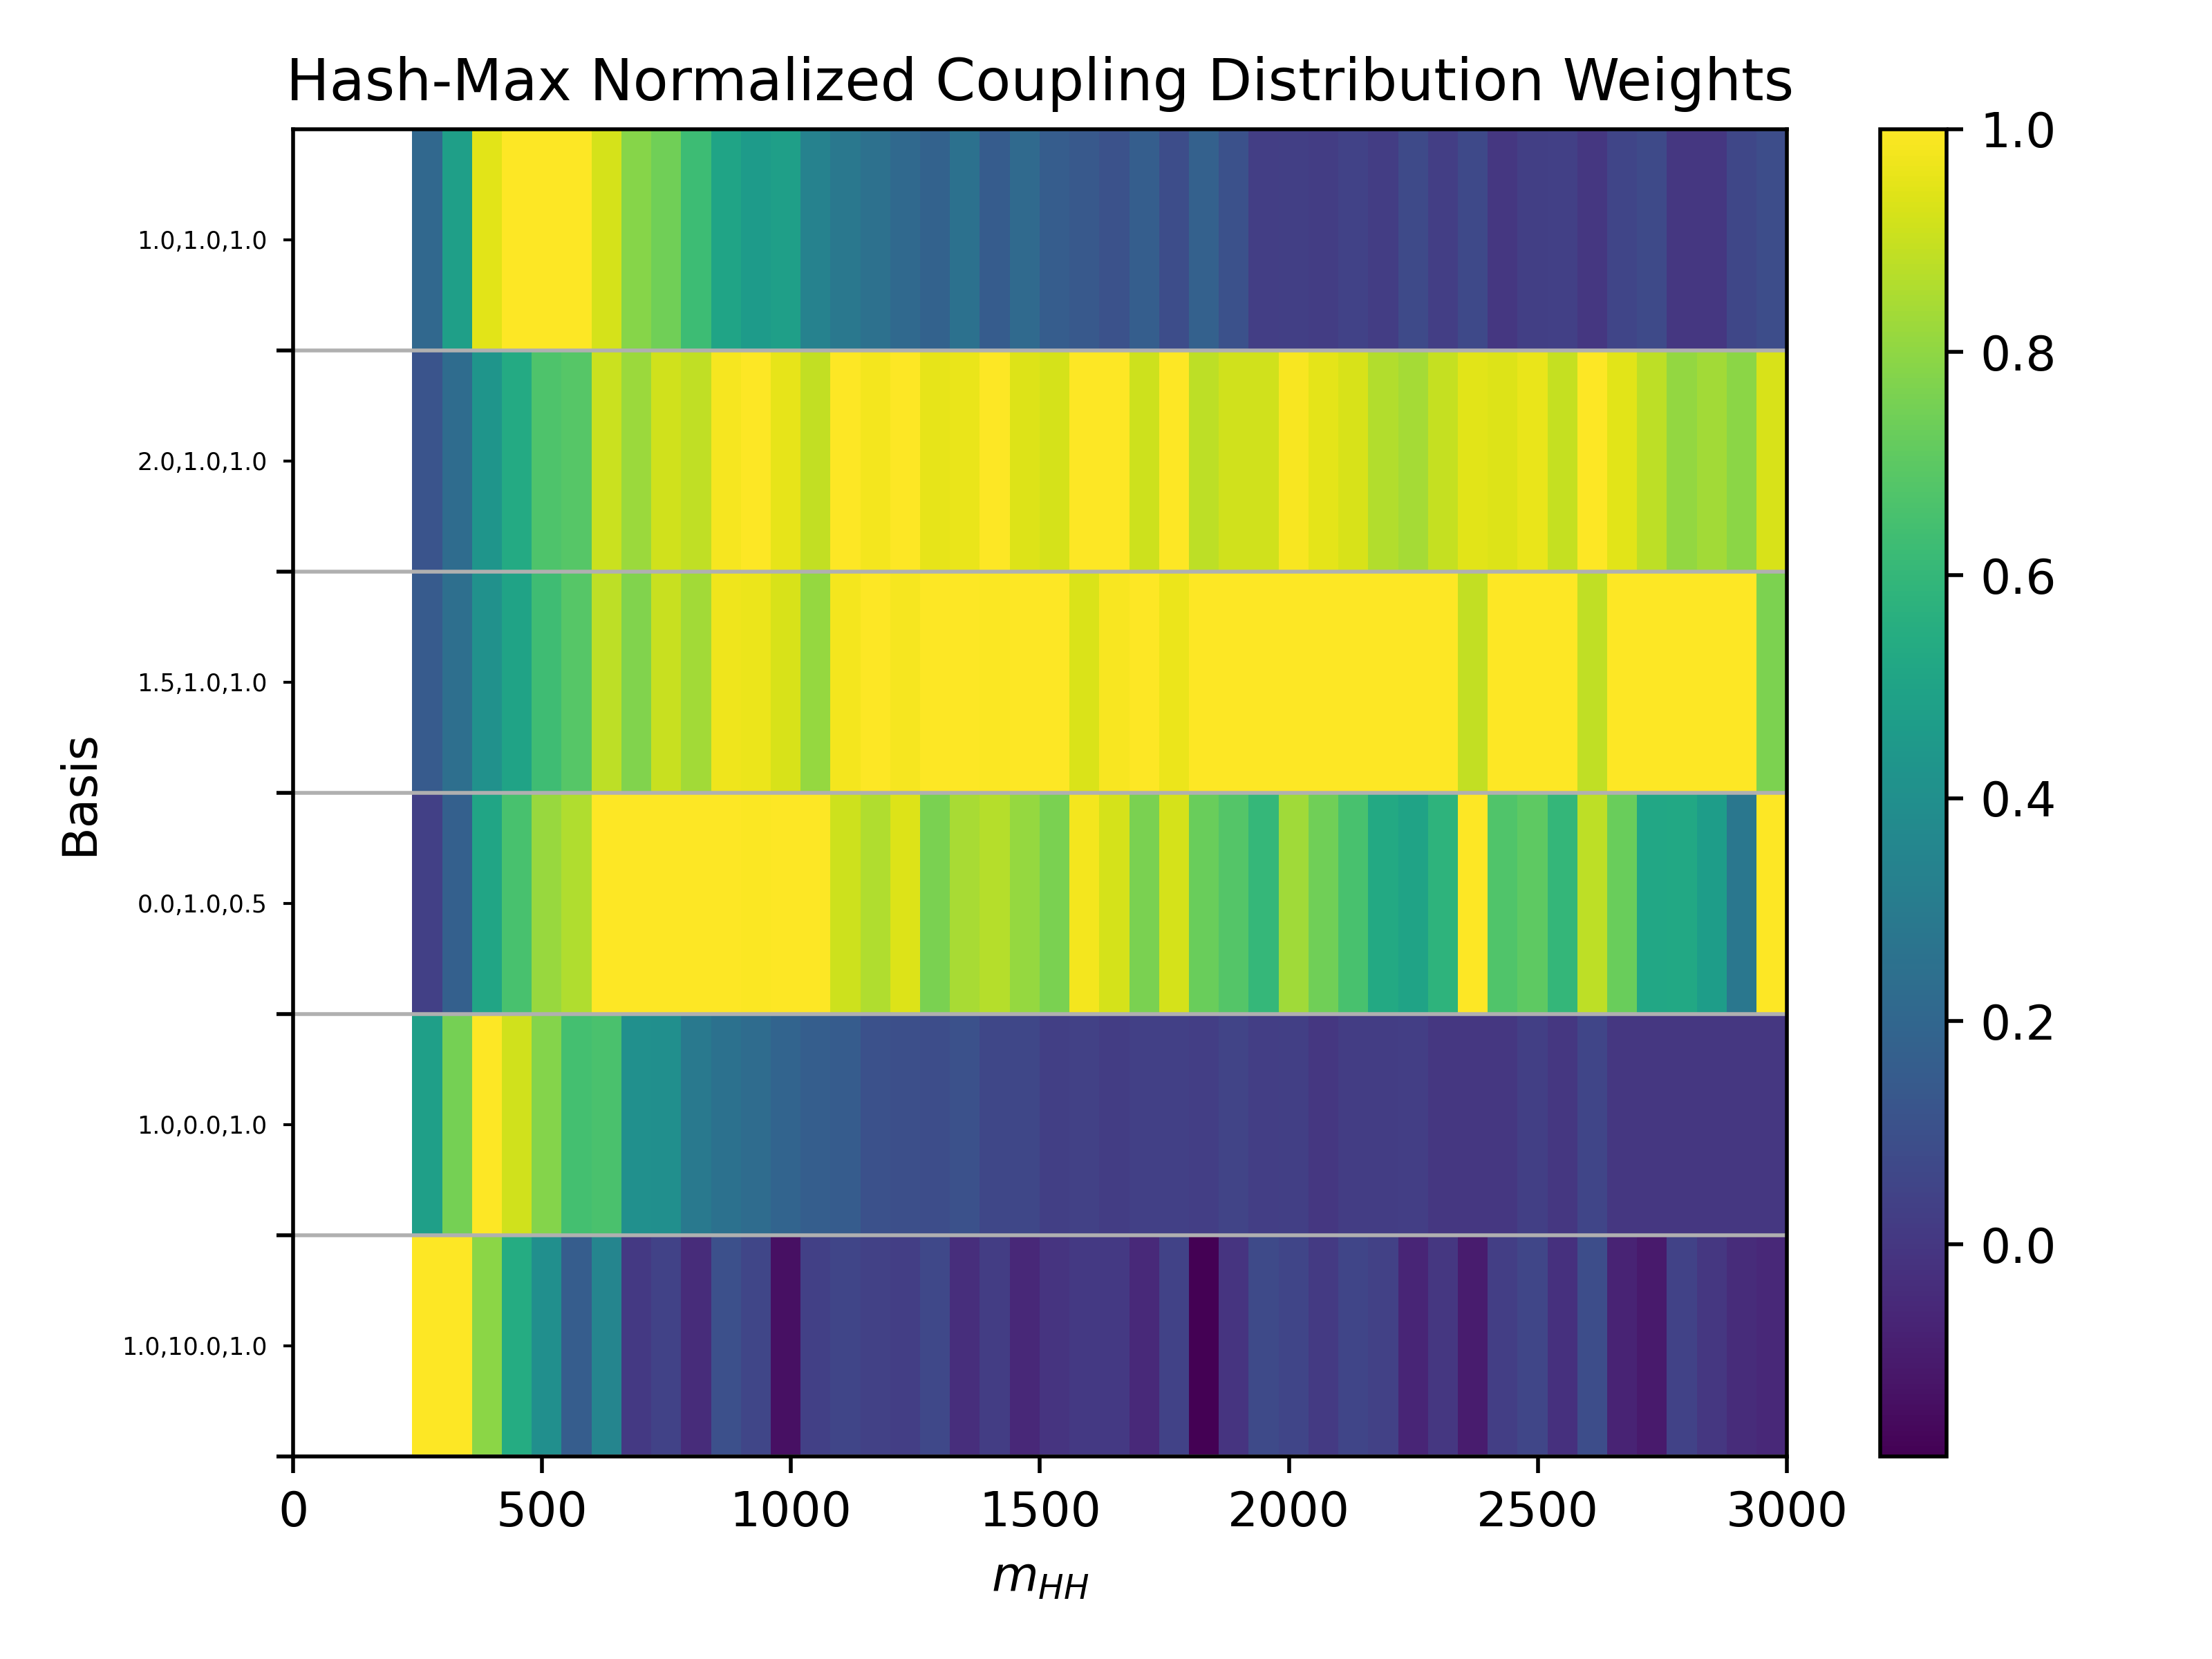
\includegraphics[width=\linewidth,height=\textheight,keepaspectratio]{coupling_scan_auto_chosen_reco_R0_hash_max}
    \end{figure}
    \end{column} \end{columns}
}

\displayonelarge{Negative Weights}{
    Negative weights can appear in the $m_{HH}$ combination. These are unphysical and should be avoided.
}{reco_mHH_cvv1p0cl2p0cv1p0}

\displayonelarge{Extreme Negative Weights}{
    In further regions of the $\kappa$ parameter space, these negative weights can be become dangerously common.
}{preview_reco_mHH_cvv0p0cl-9p0cv1p0_old}

\displayonelarge{Ranking Basis by Negative Weight Integral}{
    Take the surface integral of the number of negative bins at each point at in the $\kappa$ parameter space (mutliplying by the $\kvv \times \kl$ ``area")
}{negative_weights_rank027}

\displaythree{Negative-Weight Map of Different Bases}{
    Other bases show considerable improvement in the number of negative bins
}
{negative_weights_rank027}
{negative_weights_rank015}
{negative_weights_rank000}

\displayonelarge{Minimal Negative Weight Basis}{
    \begin{center} 
        \resizebox{0.3\textheight}{!}{\begin{tabular}{ |l|l|l| }
            \hline
                \textbf {$\kappa_{2V}$} & \textbf {$\kappa_\lambda$} & \textbf {$\kappa_V$} \\
            \hline
                1   & 1   & 1   \\ 
                0   & 1   & 0.5 \\
                1   & 0   & 1   \\ 
                1   & 10  & 1   \\ 
                0.5 & 1   & 1   \\ 
                4   & 1   & 1   \\ 
            \hline
    \end{tabular}} \end{center}
}{negative_weights_rank000.png}

\displayfour{Using Minimal Negative Weight Basis}
{reco_mHH_cvv1p0cl2p0cv1p0}
{reco_mHH_new_cvv1cl2cv1}
{preview_reco_mHH_cvv0p0cl-9p0cv1p0_old}
{preview_reco_mHH_new_cvv0cl-9cv1}


\displaytwocaption{Limits with Negative-Weight Integral Rank-1 Basis}{
    Fewer negative weights results in a much more ``natural" limit boundary.

    Sharp edges and corners appear to have been a consequence of poor signal modelling.
}
{2D_scan_2D_scan_test01_noMC16e_samps_vbf_pd_1617_c1v1.0_exclusion}
{Using old basis}
{2D_scan_2D_scan_test02_newBasis_samps_vbf_pd_1617_c1v1.0_exclusion}
{Using new basis}


    % Discound orthogonality and acceptance
    \announcesection{Why are Some Combinations Better than Others?}
\frame{
    \frametitle{``Orthogonality"}

    \begin{itemize}
        \item While this is often discussed, it's unclear (to me) what this actually means.
        \item I'm not sure if these samples genuinely span a linear space,
        \item I've never seen a discussion of what their \textit{bilinear form} (scalar product) actually is.
        \item Without the bilinear form, testing orthogonality is moot.
        \item I've discussed this with VBF theorist Christoph Englert;
        \begin{itemize}
            \item He largely dissuaded the use of orthogonality here
            \item Described the term as misused in this context (linearly independent is more appropriate)
            \item Deemed the idea as irrelevant to the topic of finding a good combination of samples
        \end{itemize}
        \item If continued research on this topic is desired, I'll need to discuss with experts further
    \end{itemize}
}

\fullscreenimage{Acceptance X Efficiency}{accXeff_explain}

\frame{
    \frametitle{Acceptance X Efficiency of Samples}

    \begin{center} 
    \begin{tabular}{ |l|l|l|c| }
        \hline
        $\kappa_{2V}$ & $\kappa_\lambda$ & $\kappa_V$ & Acc X Eff \\
                      &                  &            & (X $10^{-5}$) \\
        \hline
            4.0 &  1.0   & 1.0   & 6.80 \\
            0.0 &  1.0   & 0.5   & 6.78 \\
            2.0 &  1.0   & 1.0   & 6.18 \\
            0.0 &  1.0   & 1.0   & 5.75 \\
            1.5 &  1.0   & 1.0   & 5.54 \\
            0.5 &  1.0   & 1.0   & 4.52 \\
            1.0 &  0.0   & 1.0   & 1.59 \\
            1.0 &  10.0  & 1.0   & 1.45 \\
            1.0 &  1.0   & 1.0   & 1.41 \\
            1.0 &  2.0   & 1.0   & 0.97 \\
        \hline
    \end{tabular}
    \end{center}
}

\displayonelarge{Basis Performance VS Consitutuent Sample Acceptances}{
    { \tiny
    Each row is a basis (ordered from best performing to worst) \vspace{3mm} \\
    Each column is a sample in that basis (ordered highest to lowest) \vspace{3mm} \\
    No obvious pattern (that I can see) between acceptances and basis performance
    \par }
}{Nweight_acceptance_dump}

\displayonelarge{Acceptance X Efficiency and Basis Performance}{
    AccXeff seems to have no significant effect on the choice of one basis over another, at least with current samples (may just indicate that AccXeff doesn't vary much across the current 4b samples).
}
{Nweight_integral_VS_accXeff_sum}


    % 1) show product of coefficients and sample, elaborate on why it's bad for these to be too different
    % 2) show formula for Solidarity, alongside a heatmap for some basis
    % 3) show correlation scatter plot between sol and nWeight
    % 4) show correlation scatter plot between theoretical sol and nWeight
    % 5) show brute force dump of projected "best samples"
    \announcesection{Let's Try Something Else}

\frame{
    \frametitle{Closer Look at How Combination is Done}
    {\footnotesize
        The long polynomial functions are just coefficients $c_i(\kvv,\kl,\kv)$ to the x-secs $|A_i|^2 = \sigma_i$
        The linearly combined signal distribution $\tilde{\sigma}(\kvv,\kl,\kv)$ can be viewed more simply as:

    }
    \vspace{5mm}

    $ \tilde{\sigma}(\kvv,\kl,\kv) = $
    \vspace{3mm}
    \begin{columns}
        \begin{column}{0.55\textwidth}
            \resizebox{0.8\textwidth}{!}{ \begin{minipage}{1.0\textwidth}
            {\tiny $
    \left(2 \kappa_{2V}^{2} - \frac{124 \kappa_{2V} \kappa_{V}^{2}}{9} + \frac{61 \kappa_{2V} \kappa_{V} \kappa_{\lambda}}{9} + \frac{106 \kappa_{V}^{4}}{9} - \frac{17 \kappa_{V}^{3} \kappa_{\lambda}}{3} - \frac{\kappa_{V}^{2} \kappa_{\lambda}^{2}}{9}\right) \left|{A{\left(1,1,1 \right)}}\right|^{2} +
$

$
    \left(2 \kappa_{2V}^{2} - 8 \kappa_{2V} \kappa_{V}^{2} + 3 \kappa_{2V} \kappa_{V} \kappa_{\lambda} + 6 \kappa_{V}^{4} - 3 \kappa_{V}^{3} \kappa_{\lambda}\right) \left|{A{\left(2,1,1 \right)}}\right|^{2} +
$

$
    \left(- 4 \kappa_{2V}^{2} + 20 \kappa_{2V} \kappa_{V}^{2} - 8 \kappa_{2V} \kappa_{V} \kappa_{\lambda} - 16 \kappa_{V}^{4} + 8 \kappa_{V}^{3} \kappa_{\lambda}\right) \left|{A{\left(1.5,1,1 \right)}}\right|^{2} +
$

$
    \left(16 \kappa_{2V} \kappa_{V}^{2} - 16 \kappa_{2V} \kappa_{V} \kappa_{\lambda} - 16 \kappa_{V}^{4} + 16 \kappa_{V}^{3} \kappa_{\lambda}\right) \left|{A{\left(0,1,0.5 \right)}}\right|^{2} +
$

$
    \left(\frac{4 \kappa_{2V} \kappa_{V}^{2}}{5} - \frac{4 \kappa_{2V} \kappa_{V} \kappa_{\lambda}}{5} + \frac{\kappa_{V}^{4}}{5} - \frac{3 \kappa_{V}^{3} \kappa_{\lambda}}{10} + \frac{\kappa_{V}^{2} \kappa_{\lambda}^{2}}{10}\right) \left|{A{\left(1,0,1 \right)}}\right|^{2} +
$

$
    \left(- \frac{\kappa_{2V} \kappa_{V}^{2}}{45} + \frac{\kappa_{2V} \kappa_{V} \kappa_{\lambda}}{45} + \frac{\kappa_{V}^{4}}{45} - \frac{\kappa_{V}^{3} \kappa_{\lambda}}{30} + \frac{\kappa_{V}^{2} \kappa_{\lambda}^{2}}{90}\right) \left|{A{\left(1,10,1 \right)}}\right|^{2}
$
}
            \end{minipage}}
        \end{column}
        \begin{column}{0.05\textwidth}
            \rightarrow
        \end{column}
        \begin{column}{0.4\textwidth}
            { \small
                $c_1(\kvv,\kl,\kv) \times \sigma(1,1,1   ) +$\\
                $c_2(\kvv,\kl,\kv) \times \sigma(2,1,1   ) +$\\
                $c_3(\kvv,\kl,\kv) \times \sigma(1.5,1,1 ) +$\\
                $c_4(\kvv,\kl,\kv) \times \sigma(0,1,0.5 ) +$\\
                $c_5(\kvv,\kl,\kv) \times \sigma(1,0,1   ) +$\\
                $c_6(\kvv,\kl,\kv) \times \sigma(1,10,1  )  $\\
            \par }
        \end{column}
    \end{columns}
}


\frame{
    \frametitle{Closer Look at How Combination is Done}

    $ \tilde{\sigma}(\kvv,\kl,\kv) = $

    { \small
        \hspace{20pt} $c_1(\kvv,\kl,\kv) \times \sigma(1,1,1   ) +$\\
        \hspace{20pt} $c_2(\kvv,\kl,\kv) \times \sigma(2,1,1   ) +$\\
        \hspace{20pt} $c_3(\kvv,\kl,\kv) \times \sigma(1.5,1,1 ) +$\\
        \hspace{20pt} $c_4(\kvv,\kl,\kv) \times \sigma(0,1,0.5 ) +$\\
        \hspace{20pt} $c_5(\kvv,\kl,\kv) \times \sigma(1,0,1   ) +$\\
        \hspace{20pt} $c_6(\kvv,\kl,\kv) \times \sigma(1,10,1  )  $\\
    \par }
    \vspace{5mm}

    { \footnotesize
        Neither the coefficients nor the xsecs can be looked at in isolation; they must be viewed \textit{together} as a combined product.
        \vspace{3mm}

        If the \textit{magnitude} of some $c_i\sigma_i$ products are disproportionately large for some $\kappa$ value,
        then the smaller $c_i\sigma_i$ (and their associated sample) barely contribute to the combined signal.
        \vspace{3mm}

        The combination depends on \textit{all} six samples.
        All six samples should be contributing at all points (no slackers!).
    \par }
}


\displaytwo{The Metric of Solidarity}{
    Define measure of ``closeness" of $c_i\sigma_i$ terms:
    \vspace{3mm}

    \textit{Solidarity}, $S \equiv \frac{ \sum\limits_{i=1}^6 c_i\sigma_i }{ \textrm{Stdev}(|c_i\sigma_i|) } $
    \vspace{3mm}

     {\tiny
        i.e. take the standard deviation of the \textit{absolute values} of the $c_i\sigma_i$ products,

        normalize this by their sum (the modeled x-sec at that point),

        and then take the \textit{reciprocal} of this normalized standard deviation ($S$ increases as standard deviation gets smaller).
        \par
    }


}{contribution_maxrank01}{negative_weights_toprank000}

\displayonelarge{Correlation Between Negative Weights and Solidarity}{
    Take the surface integral of the Solidarity map for every basis to produce a ``solidarity integral", and compare to Nweight Integral.
    \vspace{5mm}

    Higher Solidarity values \textit{strongly} correlate to fewer instances of negative weights
}{Nweight_integral_VS_reco_solidarity_integral}
\displayonelarge{Correlation Between Negative Weights and Theoretical Solidarity}{
    While looser, the correlation holds even when using only the VBF->HH->4b theoretical cross-section values
    \small{(NO MONTE-CARLO)}.
    \vspace{5mm}

    Can possibly be used to predict future MC productions. Further study needed.
}{Nweight_integral_VS_theory_solidarity_integral}



    %Conclusion; Mention that systematics *still* don't work for some reasons...
    \frame{
        \frametitle{Conclusion}
        \begin{itemize} {
            \item Choice of basis can have drasitic impacts on signal modelling and final limits
            \item New (nWeight) basis optimization metric reveals poor performance of old basis
            \item Unsure of how or even if to look further into orthogonality
            \item Acceptance X Efficiency,
                at least in the current 4b samples,
                seems to have no impact on overall performance of basis
            \item ``Solidarity" metric however appears to be very effective at determining basis performance
            \item New VBF samples have finished processing. Expect more extensive studies with new samples soon.
        } \end{itemize}
    }

    \announcesection{Backup}
    \fullscreenimage{}{preview_reco_mHH_cvv0cl1cv1}
    \fullscreenimage{}{preview_reco_mHH_cvv0cl-9cv1}
    \fullscreenimage{}{preview_reco_mHH_cvv0p5cl13cv1}
    \fullscreenimage{}{preview_reco_mHH_cvv0p5cl1cv1}
    \fullscreenimage{}{preview_reco_mHH_cvv1cl10cv1}
    \fullscreenimage{}{preview_reco_mHH_cvv1cl1cv1}
    \fullscreenimage{}{preview_reco_mHH_cvv1cl2cv1}
    \fullscreenimage{}{preview_reco_mHH_cvv1p5cl-9cv1}
    \fullscreenimage{}{preview_reco_mHH_cvv2cl10cv1}
    \fullscreenimage{}{preview_reco_mHH_cvv2cl1cv1}
    \fullscreenimage{}{preview_reco_mHH_cvv4cl1cv1}
    \fullscreenimage{}{Nweight_integral_VS_theory_effective_stats_integral}
    \fullscreenimage{}{Nweight_integral_VS_reco_effective_stats_integral}
    \fullscreenimage{}{Nweight_integral_VS_accXeff_geometric}
    \fullscreenimage{}{Nweight_integral_VS_accXeff_harmonic}
    \fullscreenimage{}{Nweight_integral_VS_accXeff_sigma}
    \fullscreenimage{}{Nweight_integral_VS_accXeff_sum}

\end{document}
